\documentclass[12pt,letterpaper]{article}
\usepackage[utf8]{inputenc} 		%Codificacion del texto (ISO Latin1 encoding)
\usepackage{fancyhdr} 			%Permite acomodar a tu gusto la parte de arriba y abajo del documento
\usepackage[spanish]{babel} 		%Permite definir el idioma del dcumento
\usepackage{graphicx} 			%Permite exportar imagenes en formato eps
\usepackage{url} 			%Tipo de fuente para correos y paginas
\usepackage{pgf}
\usepackage{fleqn}
\usepackage{amssymb}
\usepackage{amsmath}
\usepackage{fancyvrb}
\usepackage{sectsty}
\usepackage{makeidx}
\usepackage{colortbl} 			%Permite colocar colores a las tablas
\usepackage{booktabs}
\usepackage{tabularx}
\usepackage{listings}
\usepackage{moreverb}
\usepackage[final]{pdfpages}
%%%%%%%%%%
%Margenes%
%%%%%%%%%%
\parskip 1mm 				%Espacio entre parrafos

%\setlength{\topmargin}{0pt}
\topmargin      0cm
\oddsidemargin	0cm  			% Ancho Letter 21,59cm
\evensidemargin 0.5cm  			% Alto  Letter 27,81cm
\textwidth	17cm
\textheight	21.0cm
\headsep	4 mm
\parindent	0.5cm
%%%%%%%%%%%%%%%%%%%%%%
%Estilo del documento%
%%%%%%%%%%%%%%%%%%%%%%
\pagestyle{fancyplain}

%%%%%%%%%%%%%%%%%%%%%%%%%%%%%%%%%%%%%%%%%%%
%Fancyheadings. Top y Bottom del documento%
%%%%%%%%%%%%%%%%%%%%%%%%%%%%%%%%%%%%%%%%%%%

\lhead{Computación Científica I} 			%Parte superior izquierda
\rhead{\bf \it Presentación Final}		 	%Parte superior derecha
\lfoot{\it IV/GZ/RF/CM/2009} 				%Parte inferior izquierda.
\cfoot{} 						%Parte inferior central
\rfoot{\bf \thepage} 					%Parte inferior derecha
\renewcommand{\footrulewidth}{0.4pt} 			%Linea de separacion inferior
%\makeindex


%%%%%%%%%%%%%%%%%%%%%%%%%%%%%%%%%%%%%%%%%%%%%%%%%%%%%%%%%%%%%%%%%%%
%%%%%%%%%%%%%%%%%%%% Aqui empieza el documento %%%%%%%%%%%%%%%%%%%%
%%%%%%%%%%%%%%%%%%%%%%%%%%%%%%%%%%%%%%%%%%%%%%%%%%%%%%%%%%%%%%%%%%%

\begin{document}
\bibliographystyle{plain}
%%%%%%%%%%%%%%%%%%%%%%%%%%
%Definicion de la portada%
%%%%%%%%%%%%%%%%%%%%%%%%%%
\begin{titlepage}
    \begin{center}
	\begin{tabular}{ccc}
	     
\includegraphics[height=1.9cm]{images/utfsm}
	    & 
	    \hspace{0.2cm}
	    \begin{tabular}{c}
		Universidad Técnica Federico Santa María \\ \hline
		\hspace{8.0cm}
		\vspace{1.2cm}
	    \end{tabular}
	    \hspace{0.2cm}
	    &
            
\includegraphics[height=2cm]{images/di}
	\end{tabular}

	\vspace{1.5cm}
	%Titulo del Documento
	    \begin{tabular}{c}
		\Huge{\textbf{Informe 2}}\\\\
		\LARGE{\sc{Sistemas y Organizaciones}}\\
		\LARGE{\sc{{``Elian y Compañía''}}}
	    \end{tabular}

	\vspace{0.5cm}
	\begin{center}
		\Large{Teorías}\\
		\begin{itemize}
			\small
		        \item \textbf{Luther\ Gullick:} \emph{``PODSCORB''}\\
		        \item \textbf{Adam\ Smith:} \emph{``La Riqueza de las Naciones''}\\
		        \item \textbf{\'Emile\ Durkheim:} \emph{``Hechos sociales''}\\
		        \item \textbf{Frederick\ Taylor:} \emph{``Administración Científica''}
		        \item \textbf{Mary\ Parker\ Follet:} \emph{``El Nuevo Estado''}\\
		        \item \textbf{Chester\ Barnard:} \emph{``Influencia de factores sicológicos y sociales en la efectividad de la organización''}\\
		        \item \textbf{Fred\ Emery:} \emph{``Sistemas Sociotécnicos''}\\
		\end{itemize}

	\end{center}
	
        \vspace{1cm}

	%Nombre del (o los) autor(es)
	\begin{tabular}{cc}
	   \begin{tabular}{c}
         	\large{Rodrigo Fernández - 2673002-3}\\ 
		\large{\url{rfernand@inf.utfsm.cl}}\\
	   \end{tabular}
		&
	   \begin{tabular}{c}
         	\large{Javier Olivares - 2673043-0}\\ 
		\large{\url{jolivaro@inf.utfsm.cl}}
	   \end{tabular}
	\end{tabular}
	   \begin{tabular}{c}
		\\
         	\large{Cristi\'an Maureira - 2673030-9}\\ 
		\large{\url{cmaureir@inf.utfsm.cl}}\\
	   \end{tabular}

	% Nombre profesor asignatura
	\begin{center}
		\large{\textbf{Profesor:} Lautaro Guerra Genskowsky}
	\end{center}

        \vspace{1cm}
	%Fecha
		\large{\sc{\today}}
    \end{center}
\end{titlepage}


\tableofcontents
\newpage

\section{Introducción}
\vspace{1cm}
Por medio del presente informe se desarrollará en profundidad,
el legado del trabajo de \emph{Émile Durkheim}, analizando sus
ideas principales, rescatando así los factores negativos y positivos
de su trabajo.
\vspace{1cm}

Para tener una idea global de la importancia del personaje histórico
analizado a continuación, tenemos que comprender primeramente que es
uno de los fundadores de la sociología moderna, ya que a través de sus
esfuerzos en éste ámbito, se logró comprender con claridad las diferencias
entre la \emph{Sicología} y la \emph{Sociología}.
\vspace{1cm}

Present\'o variadas ideas basadas en el estudio de la sociedad,
entre ellas, vale destacar la del ``trabajo social'' y la idea de ``hechos sociales'', el cual mediante el método científico realizó un estudio a la sociedad, tratando de eliminar el sentimentalismo e ilusionismo, de dicho aspecto.
\vspace{1cm}

Sobre las bases de nuestro trabajo, cambiamos la estructura de los informes entregados anteriormente y los complementamos con mayor detalle,
 adem\'as de aportar con el contexto hist\'orico y filos\'ofico de la \'epoca para poder comprender mejor los antecedentes del trabajo realizado por Durkheim.
 Tambi\'en, agregamos las obras del autor junto con un peque\~no resumen de cada una de ellas.

\newpage

\newpage

\section{Desarrollo}
\subsection{Memoria Principal y Memoria Caché}

	En la primera parte de ésta serie de papers, logramos ver que 
las operaciones aritméticas más comunes, toman entre 1 a 10 ciclos de 
CPU. Sin embargo, para poder realizar estas operaciones, es necesario
 contar con el medio de almacenamiento necesario para los datos utilizados
 en cada operación, por lo que se hace primordial, tener en consideración 
el acceso a este medio. El acceso a la memoria principal puede tomar
 aproximadamente unos 300 ciclos de CPU, por lo que si se desarrollan 
algoritmos optimizados, todo el esfuerzo es en vano si el acceso a la 
memoria principal produce grandes latencias.\\\\
	Para suerte de nosotros, los diseñadores de hardware han desarrollado
 estrategias para cubrir este gran problema, para ello decidieron colocar una
 pequeña memoria en una posición muy cercana al CPU, a la cual denominan memoria
 caché, las cuales poseen una característica importante, ser extremadamente 
rápida. Con esta disposición, los datos son accesados mucho mas rápida que si
 fueran leídos desde la memoria principal. Los procesadores más modernos poseen 
dos o más niveles de caché, denominados L1,L2 y así sucesivamente, los que dan 
a tranzar entre tamaño y velocidad. Leer desde la memoria cache L1 es muy rápido
 comparado con la memoria principal, pero a su vez tiene mucha menos capacidad 
de almacenamiento.\\\\
	La principal tarea de los programadores, es entonces, lograr un 
entendimiento sólido en este aspecto, para de esta forma llegar a comprender
 en que condiciones los datos son almacenados en la memoria caché y así lograr
 asegurar que los datos que necesitemos, se encuentren en ella.

\subsection{Localidad}

Primero que todo debemos comprender que el cache funciona \emph{reteniendo los datos utilizados recientemente},
para poder obtenerlos mas rápido en una próxima situación.
Obviamente no es posible retener los datos por un tiempo indefinido,
por lo cual son retenidos el máximo tiempo posible y van a salir de la memoria cache,
solo cuando otros datos necesiten ser retenidos.

Por lo tanto el paper analizado nos plantea que una forma de reducir la frecuencia de tener que ir a la memoria principal en variadas ocasiones,
es reutilizar los datos todas las veces que sea posible posible dentro de un periodo de tiempo corto,
porque los datos seguirán estando en el cache y no tendremos que hacer todo el procedimiento de nuevo

El concepto anteriormente señalado es conocido como \emph{localidad temporal}

Como hablamos de \emph{localidad temporal},
también es necesario tocar el tema de la \emph{localidad espacial},
la cual corresponde a cuando un programa usa múltiples partes de datos que han sido guardados contiguos en un periodo corto de tiempo.
El ejemplo que el paper ilustra de localidad espacial,
facilita la comprensión, éste nos señala una simple situación de recorrer un arreglo secuencialmente.

Por otro lado el cache aprovecha la \emph{localidad espacial} recuperando y almacenando toda la secuencia de bytes contiguos,
es decir, no sólo los bytes específicos de los datos solicitados por el procesador.
\emph{¿Cuál es la idea de recuperar y almacenar toda la secuencia de bytes?}
Claramente es poder satisfacer futuras solicitudes de direcciones de memoria cercana.

Hay otra forma en la cual una \emph{localidad espacial} de programas puede mejorar el desempeño del cache,
esta se basa en aspecto del funcionamiento del cache.
Si todo fuera perfecto cualquier linea de datos podría estar en una linea de cache,
pero para poder limitar el numero de lineas que deben ser buscadas y poder conservar los tiempos de acceso al cache cortos,
el mismo cache se preocupa de limitar las lineas de cache donde pueden estar las lineas de datos.

\begin{center}
	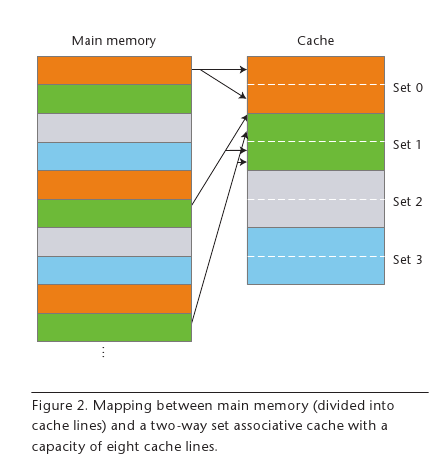
\includegraphics[scale=0.7]{images/figura2}
\end{center}

Las áreas verdes en la memoria principal pueden mapear solo una de dos lineas de cache verdes en el cache.
Si mas de dos áreas mapean el mismo conjunto,
resulta un conflicto, causando que algunos datos sean desalojados.

El conflicto de que dos áreas mapeen el mismo conjunto puede ser evitado con ayuda de la \emph{localidad espacial},
porque áreas contiguas en la memoria principal garantizan un mapeo a diferentes conjuntos en el cache.

\subsection{Mejorando la localidad espacial: \emph{Array-Merging}}
Esta Técnica, \emph{Array-Merging}, se utiliza para mejorar el tiempo de acceso a los datos en la \emph{memoria principal}.
En el ejemplo, se declaran los siguientes arreglos:
\begin{lstlisting}[language=C]
 int x[N], y[N];
 float sin6[N], cos6[N];
 int count[MAX_R];
 float g[MAX_R];
\end{lstlisting}

\begin{center}
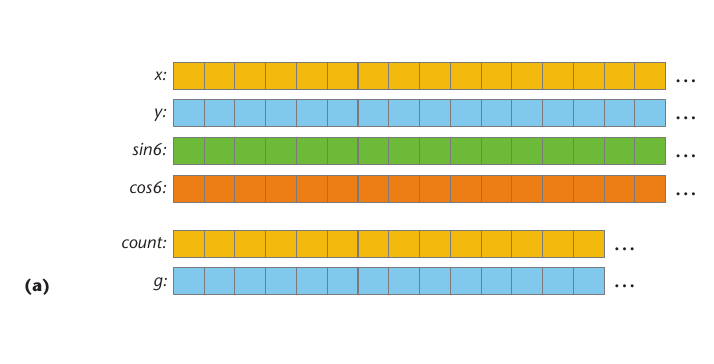
\includegraphics[scale=0.6]{images/array-1.png}
\end{center}

Si bien esto mejora el tiempo de acceso a los datos, solo sirve para requerimientos de los arreglos, ya sea $x[N]$ o $y[N]$, pero en el programa necesitamos acceso a el elemento \emph{n-esimo} de los 4 arreglos de input y el elemento \emph{r-esimo} de los 2 arreglos de output al mismo tiempo. Para mejorar la localidad espacial usamos el método del que hablamos, \emph{Array-Merging}, que guarda los valores, asociado a cada \emph{n-esimo} elemento, de forma contigua. 
Para poder llevar a cabo esta técnica podemos utilizar C, donde debemos definir estructuras donde poner cada uno de nuestros arreglos. Con esto cada vez que la memoria Cache necesite los valores, de manera anexa, también guardara los demás valores que serán necesarios. Esto lo podemos ver en el siguiente código.

\begin{lstlisting}[language=C]
struct DataStruct {
 int x, y;
 float cos6, sin6; };
DataStruct data[N];
struct AccumulationStruct {
 int count;
 float g; };
AccumulationStruct accum[Max_R];

//Now, accumulate data for all pairs of
//points (i,j).
for(i=0; i<N; ++i) //for each i < N
 for(j=i+1; j<N; ++j) { //for each j < N
  Dx = data[i].x - data[j].x;
  Dy = data[i].y - data[j].y;
  r = sqrt(Dx*Dx + Dy*Dy);
  accum[r].g += data[i].cos6 * data[j].cos6 +
   data[i].sin6 * data[j].sin6;
  ++accum[r].count;
}
\end{lstlisting}


\begin{center}
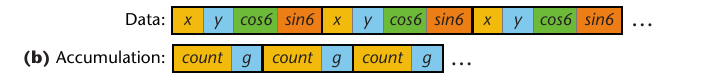
\includegraphics[scale=0.6]{images/array-2.png}
\end{center}

\subsection{Mejorando la localidad temporal: \emph{Blocking}}

La idea de mejorar la localidad temporal, es la de mantener los datos más recientemente accedidos
``cercanos'' al procesador.

El método consiste en agrupar las variables de entrada en pequeños bloques (del tamaño
\emph{blocksize}) que quepa fácilmente en el cache de menor nivel. Entonces, podemos procesar cada
par posible de puntos de esos dos bloques antes de pasar a procesar el siguiente par de bloques.
% como muestra la figura 4(...).
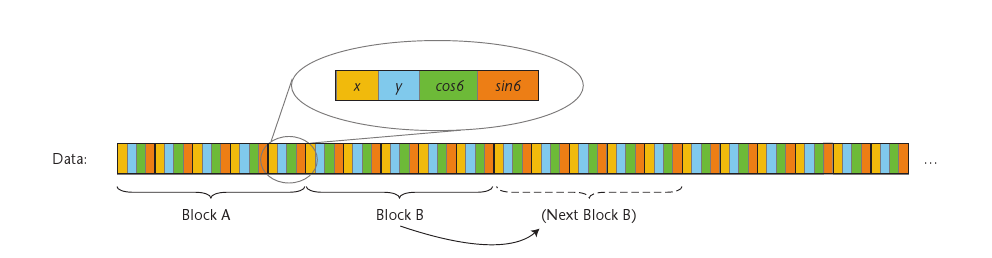
\includegraphics[scale=0.7]{images/figure4}

De esta forma, se logran realizar más computaciones por cada nuevo punto de información leído de la
memoria principal. Por ejemplo, si guardamos en el caché dos bloques de información, cada uno con un
tamaño de 100 puntos, podríamos procesar todos los 10.000 pares de puntos posibles antes de tener que
acceder al siguiente bloque de 100 puntos, lo cual es una gran mejora comparada con procesar un solo par
de puntos por cada punto leído.

La porción de código modificado queda como sigue:\\
\scriptsize
\begin{lstlisting}[language=C]
for(A = 0; A+2*blocksize < N; A+= blocksize)
	for(B=A+blocksize; B+blocksize<N; B+=blocksize)
		for(i=A; i<A+blocksize; ++i)
			for(j=B; j<B+blocksize; ++j)
			{
				(...)
			}
(...)
\end{lstlisting}
\normalsize
La desventaja de esta técnica consiste en que el código se vuelve más complejo y necesita la
implementación de más código para le manejo de nuevos casos especiales (rangos fuera de índices y evitar
que falten o se repitan operaciones).\\
 Si vemos el código, nos damos cuenta que aumentamos el número de iteraciones anidadas de 2 a 4.
Además, este no incluye los casos especiales para que funcione.\\

Por ello, nos vimos obligados a implementar nuestro própio código para probar el método de ``blocking''
en el algoritmo:
\scriptsize
\begin{lstlisting}[language=C]
	for(A=0; A<N; A+=blocksize)
	{
		C=A;
		for(B=A,flag=1; B<N; B+=blocksize,flag=0)
		{
			for(i=A; i<A+blocksize; ++i)
			{	
				if(flag)
				{
					C++;
					for(j=C; j<B+blocksize; ++j)
					{
						(...)
					}
				}
				else
					for(j=B; j<B+blocksize; ++j)
					{
						(...)
					}
			}
			C=B;
		}
	}
(...)
\end{lstlisting}
\normalsize


\textbf{Resultados}\\
En los casos de prueba  aumentó el tiempo de procesamiento en comparación con el código original.\\
Posibles causas de este resultado:
\begin{itemize}
        \item Nuestro hardware ya estaba haciendo un excelente trabajo.
        \item El aumento de operaciones por cada ciclo no se compensaba
\end{itemize}

Para más información del código utilizado, ver los anexos.

\subsection{Mejoras propuestas en nuestra investigación}
\subsubsection{Aproximación de raíces}

Utilizaremos una \emph{lookup table}, la cual es una estructura de datos, usualmente un arreglo o un arreglo asociativo.
Esta tabla es usada para reemplazar un cálculo en tiempo de ejecución,
con una simple operación de indexación de un arreglo.

Por lo tanto nos remontamos al siguiente \emph{código}:

\textbf{Original}
\begin{center}
\begin{lstlisting}[language=C]
...
for(j=i+1;j<N;++j)
{
	Dx = data[i].x - data[j].x;
	Dy = data[i].y - data[j].y;
	r = sqrt(Dx*Dx + Dy*Dy);
	accum[r].g+=data[i].cos6 + data[j].cos6 +data[i].sin6 + data[j].sin6;
	++accum[r].count;
}
...
\end{lstlisting}
\end{center}
\textbf{Modificado}
\begin{center}
\begin{lstlisting}[language=C]
...
for(j=i+1;j<N;++j)
{
	Dx = data[i].x - data[j].x;
	Dy = data[i].y - data[j].y;
	root(Dx*Dx + Dy*Dy, r)
	accum[r].g+=data[i].cos6 + data[j].cos6 +data[i].sin6 + data[j].sin6;
	++accum[r].count;
}
...
\end{lstlisting}
\end{center}

Nuestra función \emph{root()} la hemos implementado aparte en un archivo \emph{.h};
el cual no es nada más que un \emph{switch} con muchos \emph{case}.

\begin{center}
\begin{lstlisting}[language=C]
#define root(x,y)
	switch(x){
	case 0: y = 0; break;
	case 1: y = 1; break;
	case 2: y = 1; break;
	case 3: y = 1; break;
	...
	case 997: y = 31; break;
	case 998: y = 31; break;
	case 999: y = 31; break;
	}
\end{lstlisting}
\end{center}

Lo cual nos sirve para poder acceder a \emph{aproximaciones} de valores,
en vez de tener que calcular la raíz de un determinado numero.

Obviamente en la vida real,
se utilizan tablas mucho mas grandes.


\subsubsection{Aproximación de funciones trigonométricas}
Como en nuestro código realizamos muchos cálculos de \emph{funciones trigonométricas},
tenemos como motivación poder optimizar el tiempo y cálculo de éstas.

Podemos recordar las \emph{Series de Taylor}, para realizar una suerte de aproximación.

$$\sin{x} = \sum^{\infty}_{n=0} \frac{(-1)^n}{(2n+1)!} x^{2n+1} = x - \frac{x^3}{3!} + \frac{x^5}{5!} - \ldots \forall x$$

El problema radica en que algunos computadores, no pueden calcular el \emph{seno} de un valor dado,
pues están limitados a realizar operaciones básicas.

Las series de Taylor nos brindan una herramienta para poder calcular ciertas funciones trigonométricas,
con una gran presición.

Ocuparemos entonces una aproximación para calcular el \emph{seno}:

$$\sin{x} \approx x - \frac{x^3}{6} + \frac{x^5}{120} - \frac{x^7}{5040}$$

Pero, ocupamos muchas multiplicaciones para calcular los $x^k$,
por lo cual utilizaremos el \emph{Algoritmo de Horner}.

Éste algoritmo plantea una forma de calcular eficientemente polinomios de una forma monomial,
es decir,
$$ p(x) = a_0 + a_1 x + a_2 x^2 + a_3 x^3 + \cdots + a_n x^n $$

Por lo tanto podremos reducir nuestro polinomio:
$$\operatorname{sin}(x) \approx x - \frac{x^3}{6} + \frac{x^5}{120} - \frac{x^7}{5040}$$
		a,
$$\operatorname{sin}(x) \approx x \left( 1 - x^{2}\left(\frac{1}{6} + x^{2}\left(\frac{1}{120} - \frac{x^2}{5040}\right)\right)\right)$$

Si nos damos cuenta estamos reduciendo el número de multiplicaciones de 12 a 3

Luego de varias pruebas en el cálculo de efectuar ésta operación,
nos dimos cuenta que se transforma en un cálculo muy caro,
especialmente para procesadores lentos.

\subsection{Pruebas}
\subsubsection{Justificación}

Actualmente casi todos contamos con computadores con una capacidad respetable en comparación a las últimas tecnologías existentes,
pero estamos descuidando un área muy popular, los cuales son los sistemas embebidos.

Es por eso que en nuestro trabajo hemos optado por trabajar con un equipo con arquitectura ARM\footnote{http://es.wikipedia.org/wiki/ARM},
pues su capacidad de procesamiento es mucho menor, pero aspira alcanzar procesamientos al mismo nivel que un computador normal.
Si nos damos cuenta, la mayoría de los dispositivos como celulares, pocketpc, netbooks, etc, poseen poca memoria y necesitan que cada operación que se realice
sobre ella sea lo más óptima posible.

Finalmente,
una mejora en un algoritmo en un computador de escritorio o notebook actual, quizás no podremos notar la diferencia,
pero en sistemas embebidos pueden significar un gran ahorro de tiempo y provocar un mayor desempeño.

\subsubsection{Hardware}

	El kit de desarrollo Intrinsyc's Cerf$^{TM}$Board 250 provee una plataforma 
flexible, con hardware y software de alto desempe\~no para desarrollar aplicaciones 
embebidas en forma r\'apida. El kit incluye:

\begin{itemize}
	\item Intel PXA250 (XScale)
	\item Tarjeta de expansi\'on Cerf IO 250
	\item Tarjeta de expansi\'on CerfComm 250
	\item Intrinsyc's I-Linux con kernel 2.4
\end{itemize}

\begin{center}
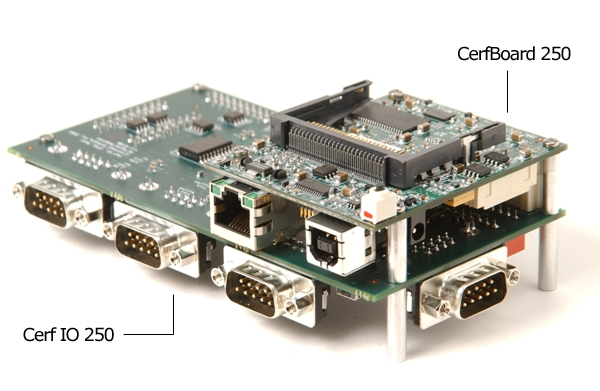
\includegraphics[scale=0.3]{images/board}
\end{center}

\subsubsection{Intel PXA250 (XScale)}

	El Intel PXA250 es un microprocesador basado en un n\'ucleo Intel XScale.
Intel XScale es una micro arquitectura RISC de 32-bit basado en una arquitectura ARM. Dise\~nado para un alto desempe\~no a costa de usar poca energ\'ia. Incorpora un conjunto completo de sistemas y perif\'ericos, funciones que le permite ser utilizado en una variedad de port\'atiles de mano.

	Posee las siguientes caracter\'isticas t\'ecnicas:

\begin{itemize}
	\item Frecuencia de 400MHz
	\item Memoria Principal de 64MB
	\item Cach\'e de instrucciones de 32KB
	\item Cach\'e de datos de 32KB
	\item B\'ufer de 256 bit
	\item Controlador de memoria basado en una arquitectura de memoria unificada, donde todos los dispositivos de memoria externos comparten un bus de direcci\'on y datos en com\'un.
	\item El controlador de memoria consiste en cuatro unidades de control principal para dar interfaz a memorias din\'amicas (SDRAM), memorias est\'aticas (ROM, SRAM, Flash), PCMCIA y chips similares.
	\item La memoria externa es vista como una colecci\'on lineal de bytes numerados desde 0 hacia adelante.
\end{itemize}

\begin{center}
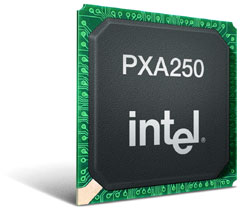
\includegraphics[scale=0.5]{images/pxa250}
\end{center}

\subsubsection{Tarjeta de expansi\'on Cerf IO 250}

	La tarjeta de expansi\'on Cerf IO 250 es una placa con entrada y salida
de propósito general. Viene equipada con un puerto serial de depuraci\'on RS232,
dos puertos seriales RS232, un puerto serial RS422/485, entre otros.

\subsubsection{Tarjeta de expansi\'on CerfComm 250}

	La tarjeta de expansi\'on CerfComm 250 est\'a equipada con caracter\'isticas
en la comunicaci\'on, viene con un controlador USB Host, un puerto Ethernet  10/100
 y tres puertos seriales de depuraci\'on RS232.

\subsubsection{Resultados}

	Para la realización de las pruebas consideramos una cantidad de datos 
igual a 50000, por otro lado programamos dos ejemplos, el primero de ellos consiste 
en la implementación mas rápida de codificar, sugerida por los papers, mientras 
que el segundo ejemplo incluye las optimizaciones sugeridas,
a continuación los resultados:\\

\begin{tabular}{|l|l|l|l|l|}
\hline
& Normal & Optimización 1 & Optimización 2 & Optimización 3 \\
\hline
Tiempo ejecución [s] & 143 & 55 & 54 & 54\\
\hline
\end{tabular}

\begin{itemize}
	\item Optimización 1: Calculo previo de funciones trigonométricas
	\item Optimización 2: Array merging
	\item Optimización 3: Blocking
\end{itemize}



\newpage

\section{Conclusiones}
\subsection{Conclusiones Individuales}
%Conclusiones personales
Personalmente pude comprender la importancia de la sociedad en un individuo, sobre todo cuando Durkheim se refiere a que el suicidio es un hecho social y no un hecho individual,
la culpa no es del sujeto, es de la sociedad.

Otro aspecto importante es como la sociedad nos ense\~na a actuar, a pensar, todo respecto a sus mismos est\'andares, y la sociedad castiga muy duramente a quien no act\'ua como
ella misma le ense\~no, un aspecto muy claro que se puede apreciar mirando una cultura determinada, el extremismo y como muchas personas viven con sus ojos vendados, aceptando
una verdad local, que a los ojos del resto del mundo puede estar erroneo, pero ?`No es el resto del mundo otra macro-cultura que también nos obliga a pensar de una forma?

Principalmente, pude darme cuenta que la visi\'on que ten\'ia Durkheim con respecto a la sociedad, fue una marca intachable en la historia del pensamiento humano,
ya que el separandose de todos los aspectos posibles, dejando atr\'as emociones, prejuicios, creencias, pudo generar un juicio imparcial para poder formar o declarar
la sociolog\'ia actual como una ciencia, que hoy en d\'ia es una de las ciencias mas importantes para el estudio de la humanidad

Finalmente, a nivel  personal me llamo mucho la atenci\'on como pudo tener la valent\'ia en su tiempo de poder analizar fen\'omenos sociales, sin ninguna influencia tan notoria
dejando de lado pensamiento que ven\'ian de 8 generaciones antes que el a nivel familiar, y que si nos damos cuenta claramente son la estructura de la organizaci\'on llamada sociedad.
Sin dejar de lado, la capacidad que tuvo para poder describir que una organizaci\'on se puede llevar a la autodestrucci\'on (Anomia), t\'ermino que sirvi\'o y sirve notablemente al
momento de analizar los riesgos de las organizaciones actuales.



\subsection{Conclusiones Generales}
%Conclusiones 'en conjunto' ......

La visi\'on de Durkheim de la sociedad marc\'o al pensamiento mundial en una manera que era
muy necesaria, dejar de lado todo tipo de prejuicios y emociones para generar un juicio imparcial y
racional de \'esta se volvio el pilar de la Sociolog\'ia, ciencia que hoy en dia se ha establecido como
una de las mas importantes de las Ciencias Sociales.

A trav\'es de las ideas del autor, las empresas se pueden analizar con ``sangre fr\'ia'', extrapolan-
do las ideas de ``hechos sociales'' y ``estructura'' a organizaciones mas pequeñas. De esta manera se
puede entender mejor la forma de comportarse de algunas organizaciones que tienden
a la autodestrucci\'on o que logran surgir en ambientes altamente hostiles.

%	\item Sobre los hechos sociales
Adem\'as, cuando uno es insertado en una nueva comunidad, como lo es una organizaci\'on o empresa hoy en d\'ia, uno 
se ve rodeado de un sistema con una cultura propia y muchas veces diferente a la del individuo. Estos 
detalles impl\'icitos muchas veces dentro dela organizaci\'on, son los reconocidos como ``hechos sociales''
por Durkheim. Por ello, podemos concluir que fue importante que Durkheim halla reconocido que los 
hechos sociales deb\'ian ser analisados por m\'etodos diferentes a los de la psicolog\'ia, ya que los estudios 
de sociolog\'ia desarrollados por \'el han sido un gran aporte para el estudio de la administraci\'on general 
de estos ``sistemas humanos'', jugando un rol medular en el asunto. 

%	\item Sobre las Corrientes Sociales\\
Tambi\'en, esto dicho anteriormente  deber\'iamos encararlo con objetividad, desprendiéndonos de todos los prejuicios y preconceptos que podamos tener antes de abordarlos.\\
Esto puede llegar a ser muy difícil, si a modo de ejemplo tomamos por punto de partida que el analista pertenece a una colectividad, a una sociedad, que tiene determinado su pensamiento a través del lenguaje que determina en sí mismo una estructura preestablecida de pensamiento lógico.


%	\item Sobre la divisi\'on del trabajo social\\
Para el estudio y administraci\'on de empresas u organizaciones, el concepto de solidaridad desarrollado
por Durkheim es importante de recalcar. Vi\'endolo desde su punto de vista, cada organizaci\'on deber\'ia 
buscar una solidaridad mec\'anica entre sus miembros. De esta forma, los individuos lograr\'ian adquirir 
una mentalidad enfocada a los objetivos de la empresa (vista como comunidad), y as\'i, mantener un 
ambiente de unidad y confianza en torno a los ideales de \'esta. Es notable mencionar que muchas 
organizaciones tienden a de hoy en dia tienden a fomentar un ambiente competitivo entre sus integrantes, 
lo cual, al igual que la mentalidad individualista en la realidad actual, conlleva muchas veces a problemas 
t\'ipicos de una solidaridad org\'anica.

%	\item  Sobre la educaci\'on\\
Ahora si analizamos las las funciones de la educaci\'on destacadas por Durkheim, desde el punto de vista de las organizaciones, 
la educaci\'on sirve como herramienta para lograr un mayor orden social, una mayor lealtad y una mayor especializaci\'on 
de los integrantes hacia la comunidad, siendo as\'i de gran importancia para mejorar la integraci\'on de nuevos miembros
y el crecimiento de la empresa.
	
%	\item  Sobre el Crimen
%Durkheim identific\'o al crimen como un indicador de la necesidad de cambios dentro de las organizaciones. 

%	\item Sobre la Ley
%Postulados principales:
% Diferencia duramente entre el Individualismo y la avaricia y el egoismo
% Avaricia y egoismo no son en lo absoluto posturas morales
% Estudia la Ley como una expresi\'on que garantizaba los valores fundamentales de la sociedad.

%	\item Sobre el Suicidio\\
De la misma manera, Durkheim, con su trabajo sobre el suicidio de los individuos con diferentes hechos sociales, logra destacar como ciertos 
factores en la sociedad (debilitamiento de los lazos de integraci\'on, desregularizaci\'on moral y falta de definiciones 
leg\'itimas, sociedades muy opresivas) pueden llevar a la autodestrucci\'on de sus miembros.\\
Por ello, se puede concluir que  es importante que las organizaciones se preocupen de mantener a sus integrantes 
cuidando de no desarrollar estas fallas que requieren de una reconstrucci\'on social.

%	\item Sobre la Religi\'on\\
Por \'ultimo, sus estudios sobre la religi\'on permitieron comprender mejor el desarrollo del orden social en las primeras comunidades, 
cumpliendo estas la funci\'on de separar lo mundano o cotidiano de las cosas intangibles, que relacionadas con lo sagrado, 
lograban la generaci\'on de normas que fomentaban el orden social.



\newpage

\newpage

\section{Glosario}
\begin{description}
	\item[Memoria Principal:]
Está formada por bloques de circuitos integrados o chips capaces de almacenar, retener o ``memorizar''
información digital, es decir, valores binarios; a dichos bloques tiene acceso el microprocesador de la
computadora. El microprocesador la accede mediante el bus de direcciones. La MP es el núcleo del
sub-sistema de memoria de un computador, y posee una menor capacidad de almacenamiento que la memoria
secundaria, pero una velocidad muy superior.

	\item[Bus:]
Es un sistema digital que transfiere datos entre los componentes de un computador o
entre computadores. Están formado por cables o pistas en un circuito impreso, dispositivos como
resistencias y condensadores además de circuitos integrados. La función del Bus es la de permitir la
conexión lógica entre distintos subsistemas de un sistema digital, enviando datos entre dispositivos de
distintos ordenes: desde dentro de los mismos circuitos integrados, hasta equipos digitales completos que
forman parte de supercomputadoras.

	\item[Memoria Caché:]
Es un sistema especial de almacenamiento de alta velocidad. Puede ser tanto un área reservada de la
memoria principal como un dispositivo de almacenamiento de alta velocidad independiente. Hay dos tipos de
cache frecuentemente usados en las computadoras personales: memoria cache y cache de disco. Una memoria
cache, llamada también a veces almacenamiento cache o RAM cache, es una parte de memoria RAM estática de
alta velocidad (SRAM) más que la lenta y barata RAM dinámica (DRAM) usada como memoria principal. La
memoria cache es efectiva dado que los programas acceden una y otra vez a los mismos datos o
instrucciones. Guardando esta información en SRAM, la computadora evita acceder a la lenta DRAM.

	\item[Principio de Localidad:]
Los programas acceden una porción relativamente pequeña del
espacio de direcciones en un determinado instante de tiempo.

	\item[Localidad Espacial:]
Se refiere al espacio en donde son guardados los datos en la memoria. Es una propiedad en la que se basa
una de las políticas de extracción utilizadas para determinar cuándo y qué bloque de memoria principal
hay que traer a memoria cache. Si un item es referenciado, los items tenderán a ser referenciados a la
brevedad.

	\item[Localidad Temporal:]
Se refiere a la frecuencia con la cual son consultados ciertos bloques guardados en la memoria.
Si un item es referenciado, tenderá a ser referenciado nuevamente a la brevedad.

	\item[Latencia:]
En redes informáticas de datos se denomina latencia a la suma de retardos temporales dentro de una red.
Un retardo es producido por la demora en la propagación y transmisión de paquetes dentro de la red.

	\item[Ciclos de Reloj:]
La frecuencia de reloj indica la velocidad a la que un ordenador realiza sus operaciones más básicas,
como sumar dos números o transferir el valor de un registro a otro. Se mide en ciclos por segundo
(hercios).
	\item[CPU:]
Es el componente en una computadora digital que interpreta las instrucciones y procesa los datos
contenidos en los programas de la computadora. Las CPU proporcionan la característica fundamental de la
computadora digital (la programabilidad) y son uno de los componentes necesarios encontrados en las
computadoras de cualquier tiempo, junto con el almacenamiento primario y los dispositivos de
entrada/salida. 
\end{description}

\newpage

\section{Anexos}
\scriptsize
\subsection{C\'odigo base}
\begin{verbatimtab}
#include <math.h>
#include <stdlib.h>
#include <stdio.h>
#include "global.h"

int x[N], y[N];
float theta[N];
int count[N];
float g[(int)(N*1.5)];

int main(int argc, char **argv)
{
	for(i=0;i<N;i++)
	{
		x[i] = i;
		y[i] = i;
		theta[i] = 6*random();
	}

	//	Almacenamos tiempo capturado
	initialTime = getTime();

	//	Now, accumulate data for all pairs of
	//	points (i,j).
	for(i=0; i<N; ++i)	//for each i < N
		for(j=i+1; j<N; ++j)	//for each j < N
		{
			Dx = x[i]-x[j];
			Dy = y[i]-y[j];
			r = sqrt(Dx*Dx + Dy*Dy);
			g[r] += cos(6*(theta[i]-theta[j]));
			++count[r];
		}

	for (r = 0; r < MAX_R; r++)
		g[r] = g[r] / count[r];

	//	Calculando lo que ha tomado el calculo
	finalTime = getTime();

	//	Imprimimos resultados
	results();
	return 0;

}
\end{verbatimtab}


\subsection{C\'odigo base mejorado mejorada}
\begin{verbatimtab}
#include <math.h>
#include <stdlib.h>
#include <stdio.h>
#include "global.h"

int x[N], y[N], ii;
float theta[N];
int count[N];
float g[(int)(N*1.5)];
float sin6[N], cos6[N];

int main(int argc, char **argv)
{
	for(i=0;i<N;i++)
	{
		x[i] = i;
		y[i] = i;
		theta[i] = 6*random();
	}

	//	Almacenamos tiempo capturado
	initialTime = getTime();

	for(ii=0; ii<N; ++ii)
	{ 	
		sin6[ii] = sin(6*theta[ii]);
		cos6[ii] = cos(6*theta[ii]);
	}
	
	for(i=0; i<N; ++i)
		for(j=i+1; j<N; ++j)
		{
		Dx = x[i]-x[j];
		Dy = y[i]-y[j];
		r = sqrt(Dx*Dx+Dy*Dy);
		g[r] += cos6[i]*cos6[j]+sin6[i]*sin6[j];
		++count[r];
		}
	
	for (r = 0; r < MAX_R; r++)
		g[r] = g[r] / count[r];

	//	Calculando lo que ha tomado el calculo
	finalTime = getTime();

	//	Imprimimos resultados
	results();
	return 0;

}
\end{verbatimtab}

\subsection{C\'odigo con localidad espacial mejorada}
\begin{verbatimtab}
#include <math.h>
#include <stdio.h>
#include <stdlib.h>
#include <time.h>
#include "global.h"

struct DataStruct
{
	int x, y;
	float cos6, sin6;
} data[N];

struct AccumulationStruct
{
	int count;
	float g;
} accum[(int)(N*1.5)];

int ii;
float theta[N];

int main(int argc, char **argv)
{
	for(i=0;i<N;i++)
	{
		data[i].x = i;
		data[i].y = i;
		theta[i] = 6*random();
	}


	//	Almacenamos tiempo capturado
	initialTime = getTime();

	for (ii = 0; ii < N; ii++)
	{
		data[ii].cos6 = cos(6*theta[ii]);
		data[ii].sin6 = sin(6*theta[ii]);
	}
	
	for(i=0; i<N; ++i)	
		for(j=i+1; j<N; ++j)
		{
			Dx = data[i].x - data[j].x;
			Dy = data[i].y - data[j].y;
			r = sqrt(Dx*Dx + Dy*Dy);
			accum[r].g += data[i].cos6 * data[j].cos6 + data[i].sin6 * data[j].sin6;
			++accum[r].count;
		}

	for (r = 0; r < MAX_R; r++)
		accum[r].g = accum[r].g / accum[r].count;

	//	Calculando lo que ha tomado el calculo
	finalTime = getTime();
	
	//	Imprimimos resultados
	results();
	return 0;
}
\end{verbatimtab}

\subsection{C\'odigo con localidad espacial y temporal mejorada}
\begin{verbatimtab}
#include <math.h>
#include <stdio.h>
#include <stdlib.h>
#include <time.h>
#include "global.h"
#include "tabla.h"

struct DataStruct
{
	int x, y;
	float cos6, sin6;
} data[N];

struct AccumulationStruct
{
	int count;
	float g;
} accum[(int)(N*1.5)];

int ii;
int A,B,C,blocksize =1000;
int flag;
float theta[N];

int main(int argc, char **argv)
{
	for(i=0;i<N;i++)
	{
		data[i].x = i;
		data[i].y = i;
		theta[i] = 6*random();
	}

	//	Almacenamos tiempo capturado
	initialTime = getTime();

	for(ii = 0; ii < N; ii++)
	{
		data[ii].cos6 = cos(6*theta[ii]);
		data[ii].sin6 = sin(6*theta[ii]);
	}

	for(A=0; A<N; A+=blocksize)
	{
		C=A;
		for(B=A,flag=1; B<N; B+=blocksize,flag=0)
		{
			for(i=A; i<A+blocksize; ++i)
			{	
				if(flag)
				{
					C++;
					for(j=C; j<B+blocksize; ++j)
					{
						Dx = data[i].x - data[j].x;
						Dy = data[i].y - data[j].y;
						r = sqrt(Dx*Dx + Dy*Dy);
						accum[r].g += data[i].cos6 * data[j].cos6 + data[i].sin6 * data[j].sin6;
						++accum[r].count;
					}
				}
				else
					for(j=B; j<B+blocksize; ++j)
					{
						Dx = data[i].x - data[j].x;
						Dy = data[i].y - data[j].y;
						r = sqrt(Dx*Dx + Dy*Dy);
						accum[r].g += data[i].cos6 * data[j].cos6 + data[i].sin6 * data[j].sin6;
						++accum[r].count;
					}
			}
			C=B;
		}
	}

	for (r = 0; r < MAX_R; r++)
		accum[r].g = accum[r].g / accum[r].count;

	//	Calculando lo que ha tomado el calculo
	finalTime = getTime();
	
	//	Imprimimos resultados
	results();
	return 0;

}
\end{verbatimtab}

\newpage

\bibliography{informe}

\end{document}
